%!TEX encoding = UTF-8 Unicode
\documentclass[
    fontsize=12pt,
    headings=small,
    parskip=half,           % Ersetzt manuelles setzten von parskip/parindent.
    bibliography=totoc,
    numbers=noenddot,       % Entfernt den letzten Punkt der Kapitelnummern.
    open=any,               % Kapitel kann auf jeder Seite beginnen.
%   final                   % Entfernt alle todonotes und den Entwurfstempel.
    ]{scrreprt}

% ===================================Praeambel==================================

% Kodierung, Sprache, Patches {{{
\usepackage[T1]{fontenc}    % Ausgabekodierung; ermoeglicht Akzente und Umlaute
                            %  sowie korrekte Silbentrennung.
\usepackage[utf8]{inputenc} % Erlaub die direkte Eingabe spezieller Zeichen.
                            %  Utf8 muss die Eingabekodierung des Editors sein.
\usepackage[ngerman]{babel} % Deutsche Sprachanpassungen (z.B. Ueberschriften).
\usepackage{microtype}      % Optimale Randausrichtung und Skalierung.
\usepackage[
    autostyle,
    ]{csquotes}             % Korrekte Anfuehrungszeichen in der Literaturliste.
\usepackage{fixltx2e}       % Patches fuer LaTeX2e.
\usepackage{scrhack}        % Verhindert Warnungen mit aelteren Paketen.
% }}}

% Schriftarten {{{
\usepackage{mathptmx}       % Times. Package 'times.sty' is obsolete.
\usepackage[scaled=.92]{helvet}
\usepackage{courier}
% }}}

% Biblatex {{{
% \usepackage[
%     style=alphabetic,
%     backend=biber,
%     backref=true
%     ]{biblatex}             % Biblatex mit alphabetischem Style und biber.
% \bibliography{Literatur.bib}% Dateiname der bib-Datei.
% }}}

% Dokument- und Texteinstellungen {{{
\usepackage[
    a4paper,
    margin=2.54cm,
    marginparwidth=2.0cm,
    footskip=1.0cm
    ]{geometry}             % Ersetzt 'a4wide'.
\clubpenalty=10000          % Keine Einzelzeile am Beginn eines Paragraphen
                            %  (Schusterjungen).
\widowpenalty=10000         % Keine Einzelzeile am Ende eines Paragraphen
\displaywidowpenalty=10000  %  (Hurenkinder).
\usepackage{floatrow}       % Zentriert alle Floats.
\usepackage{ifdraft}        % Ermoeglicht \ifoptionfinal{true}{false}
\pagestyle{plain}           % keine Kopfzeilen
% \sloppy                     % großzügige Formatierungsweise
\deffootnote{1em}{1em}{\thefootnotemark.\ } % Verbessert Layout mehrzeiliger Fußnoten

\makeatletter
\AtBeginDocument{%
    \hypersetup{%
        pdftitle = {\@title},
        pdfauthor  = \@author,
    }
}
\makeatother
% }}}

% Weitere Pakete {{{
\usepackage{graphicx}       % Einfuegen von Graphiken.
\usepackage{tabu}           % Einfuegen von Tabellen.
\usepackage{multirow}       % Tabellenzeilen zusammenfassen.
\usepackage{multicol}       % Tabellenspalten zusammenfassen.
\usepackage{booktabs}       % Schönere Tabellen (\toprule\midrule\bottomrule).
\usepackage[nocut]{thmbox}  % Theorembox bspw. fuer Angreifermodell.
\usepackage{amsmath}        % Erweiterte Handhabung mathematischer Formeln.
\usepackage{amssymb}        % Erweiterte mathematische Symbole.
\usepackage{rotating}
\usepackage[
    printonlyused
    ]{acronym}              % Abkuerzungsverzeichnis.
\usepackage[
    colorinlistoftodos,
    textsize=tiny,          % Notizen und TODOs - mit der todonotes.sty von
    \ifoptionfinal{disable}{}%  Benjamin Kellermann ist das Package "changebar"
    ]{todonotes}            %  bereits integriert.
\usepackage[
    breaklinks,
    hidelinks,
    pdfdisplaydoctitle,
    pdfpagemode = {UseOutlines},
    pdfpagelabels,
    ]{hyperref}             % Sprungmarken im PDF. Laed das URL Paket.
    \urlstyle{rm}           % Entfernt die Formattierung von URLs.
\usepackage{breakurl}
\def\UrlBreaks{\do\/\do-}
\usepackage{listings}       % Spezielle Umgebung für...
    \lstset{                %  ...Quelltextformatierung.
        language=C,
        breaklines=true,
        breakatwhitespace=true,
        frame=L,
        captionpos=b,
        xleftmargin=6ex,
        tabsize=4,
        numbers=left,
        numberstyle=\ttfamily\footnotesize,
        basicstyle=\ttfamily\footnotesize,
        keywordstyle=\bfseries\color{green!50!black},
        commentstyle=\itshape\color{magenta!90!black},
        identifierstyle=\ttfamily,
        stringstyle=\color{orange!90!black},
        showstringspaces=false,
        }
% }}}

% ===================================Dokument===================================

\title{Microservices und die Zukunf von DevOps}
\author{Bennet Brunsen, Mathias Schmialek}
% \date{01.01.2015} % falls ein bestimmter Tag eingesetzt werden soll, einfach diese Zeile aktivieren

\begin{document}

\begin{titlepage}
\begin{center}\Large
    Universität Hamburg \par
    Fachbereich Informatik
    \vfill
    \makeatletter
    {\Large\textsf{\textbf{\@title}}\par}
    \makeatother
    \bigskip
    am Arbeitsbereich Softwarearchitektur (SWA) \par
    \bigskip
    \makeatletter
    {\@author} \par
    \makeatother
    \bigskip
    \makeatletter
    {\@date}
    \makeatother
    \vfill
    \vfill
\end{center}
\end{titlepage}
\newpage

\begin{abstract}
Dieses Paper fasst die Kapitel 4 und 15 des Buches "DevOps" von Len Bass et. al. zusammen. Zusätzlich wird in diesem Paper genauer auf Microservices eingegangen und wie diese im Bezug zu DevOps stehen. Die Kapitel umfassen eine kleine Einführung zu DevOps und einen Ausblick für die Zufunkt von DevOps. Gefolgt von einigen Problemen die DevOps mit sich bringen und wie diese gelöst werden können.
\end{abstract}


\tableofcontents

\section{Einleitung}
\subsection{Developer}
Viele Betriebe wie zum Beispiel Versicherungen sind heutzutage beinahe vollständig auf Software angewiesen, die ihre Arbeit korrekt abbildet und vereinfacht. Diese Software wird von Entwicklern (Developern) mit Hilfe von Abstraktion und Programmiersprachen hergestellt. Damit die Software auch den Ansprüchen der Anwender entspricht, nimmt der Entwickler die Anforderungen vom Anwender beziehungsweise dem Auftraggeber entgegen und setzt diese in Programmcode um. Zusätzlich ist es die Aufgabe des Entwicklers den geschriebenen Programmcode sowohl manuell als auch programmatisch zu testen und damit ein korrektes Verhalten der Anwendung sicherzustellen.\\
Das Ergebnis der Arbeit eines Entwicklers ist ein Stück Software, das dem Kunden als Installationsdatei oder Ähnlichem übergeben wird. Der Entwickler selbst ist nicht dafür zuständig, dass die Anwendung in den laufenden Betrieb des Kunden integriert wird.

\subsection{Operation}
Unter Operations werden im herkömmlichen Sinne Mitarbeiter mit IT-Kenntnissen verstanden, deren Ziel es ist, den täglichen IT-Betrieb am laufen zu halten. Zu ihren Aufgaben gehören unter anderem die Bereitstellung von Hardware für Mitarbeiter des Betriebes sowie die Verwaltung von Servern. Sie sind ebenfalls dafür zuständig, Software unter anderem auf die Geräte der Mitarbeiter und auf die Server des Betriebes zu spielen. Dabei kann die Software entweder käuflich erworben oder im eigenen Unternehmen entwickelt worden sein. Dies wird in der Regel mit Skripten realisiert, die Operations selber anlegen.\\
Zu einer Software, die kommerziell erworben wurde, gibt es in der Regel so gennante Service Level Agreements, die eine mit dem Softwarehersteller vereinbarte Leistungsqualität der einzusetzenden Software beschreiben. Ein Beispiel hierfür wäre, dass ein Hersteller von einer Cloudbasierten Anwendung seinem Kunden verspricht, dass die Anwendung mit einer bestimmten Anzahl an Anfragen innerhalb einer definierten Zeitspanne zurecht kommt, sodass keine Ausfälle entstehen. Innerhalb eines Betriebes überwachen Operations die Service Level Agreements und melden gegebenenfalls Verstöße ihren Vorgesetzten oder dem Hersteller der Software. \\
Um die Einhaltung der Service Level Agreements zu überprüfen, wird die Software mit Hilfe von Monitoring und Logging Werkzeugen überwacht. Dabei vermitteln die Werkzeuge des Monitorings den Operations wichtige Informationen wie zum Beispiel den Speicherverbrauch und den Status der laufenden Anwendungen. Mit Hilfe der Logging Werkzeuge, können die Operations auf Fehler innerhalb der Anwendung schließen. Für den Fall, dass die Umgebung der Anwendung falsch konfiguriert ist, wird dies üblicherweise in Log-Dateien geschrieben, die den Operations zur Verfügung stehen. \\
Wie bereits erwähnt, ist das Ziel von Operations den IT-Betrieb am laufen zu halten. Dies wird in der Regel als Business Continuity bezeichnet. Allerdings ist dies nicht nur mit einer für die Anwendung passend konfigurierten Umgebung möglich. Die Rechner und Server eines Betriebes müssen nach Außen abgesichert werden, um Ausfälle durch Schadangriffe so gut wie möglich zu unterbinden. Dies ist ebenfalls ein Aufgabenbereich von Operations.

\subsection{Agile Softwareentwicklung}
Neben der klassischen Softwareentwicklung, die nach starren Modellen wie zum Beispiel dem Wasserfallmodell arbeitet, hat sich in den letzten Jahren die agile Softwareentwicklung etabliert. Die agile Softwareentwicklung mit agilen Vorgehensweisen wie zum Beispiel Scrum oder Xtreme Programming, bindet den Kunden stärker in den Entwicklungsprozess ein und bietet die Möglichkeit schon während der Entwicklung auf das die Software Einfluß zu nehemen. \\
Len Bass hat bei der agilen Softwareentwicklung drei Phasen identifiziert, auf die im folgenden eingegangen wird. Die erste Phase ist die sogenannte Inception Phase. In dieser Phase werden unter anderem die Anforderungen an die Software aufgenommen und erste Modellierungsarbeiten betrieben. Zustäzlich wird in dieser Phase ein Release Plan erstellt, der mit dem Kunden abgestimmt wird.\\
Die zweite Phase ist die so genannte Construction Phase. In dieser Phase wird die Software nach agilen Methoden wie zum Beispiel Scrum entwickelt. Das Ergebnis dieser Phase ist ein Software Artifakt, das dem Kunden übergeben werden kann. \\
Die finale Phase ist die Transition Phase. In dieser Phase wird das zuvor hergestellte Artifakt beim Kunden auf die Rechner beziehungsweise Server gespielt und somit in den laufenden Betrieb integriert.

\subsection{Monolith}
Unter einem Monolithen wird in der Softwareentwicklung ein Architekturstil verstanden, bei dem die Software auf höchster Ebene nur als eine einzelne Komponente gesehen wird. Monolithen sind in der Regel sehr große Komponenten, die mehr als 50.000 Zeilen an Programmcode aufweisen. Darüber hinaus enthalten Monolithen die gesamte Geschäftslogik einer Anwendung. Monolithen entstehen implizit, wenn kein spezieller Architekturstil vorgegeben wird, da die Codebasis mit der Zeit durch weitere Entwicklungsarbeiten wächst. Häufig sind monolithisch entworfene Anwendungen im Serverbereich von Webanwendungen aufzufinden. \\
Anwendungen, die nach diesem Stil entworfen wurden, weisen einige Nachteile auf. Zum einen erfordert jede Änderung (zum Beispiel eine Fehlerkorrektur) ein erneutes Deployment der gesamten Anwendung. Zusätzlich skalieren monolithische Anwendung schlecht. Sollte zum Beispiel eine logische Einheit des Monolithen wie die Datenpersistierung nicht unter der aktuellen Last bestehen, müsste eine zweite Instanz der gesamten Anwendung erzeugt werden, um die Last zu bewältigen. Dies ist nicht optimal, da eigentlich nur die Datenpersistierung zusätzliche Instanzen benötigen würde. \\
Ein weiterer Nachteil, der durch die monolithische Architektur entsteht, findet sich im Release einer neuen Version wieder. Da bei einem erneuten Deployment die gesamte Anwendung erneut auf die Rechner beziehungsweise Server gespielt werden muss, sind diese in der Zeit des Deployments nicht verfügbar. Dies kann je nach Anwendungsfeld zu einem Ausfall an Einnahmen führen. Zum Beispiel könnte ein Händler im Internet keine Produkte verkaufen, während seine Anwendung nicht verfügbar ist. Aus diesem Grund werden neue Versionen einer monolithischen Anwendung so selten wie nötig auf die Systeme gespielt. Dies führt wiederum dazu, dass eine neue Version nicht bei jedem neuen Feature entsteht, sondern erst mit einer Vielzahl neuer Features. Die vielen neuen Features können allerdings Inkompatibilitäten in der Anwendung erzeugen sowie zu einer erhöhten Ferleranfälligkeit führen. Daher erfoderdet eine neue Version einen sehr hohen Aufwand beim Testen der Anwendung. Darüber hinaus kann eine neue Version auch eine völlig anders konfigurierte Umgebung erfordern, was den Aufwand einer neuen Version ebenfalls erhöht. All dies erfordert einen sehr hohen Koordinationsaufwand und eine langfristige Planung, was wiederum zu einem langsamen Release der Anwendung führt.

\chapter{DevOps}
Unter dem Begriff DevOps werden eine Menge an Maßnahmen, die die Bereiche Development und Operations enger zusammenführen, verstanden. In diesem Kapitel wird zunächst die Motivation von DevOps beschrieben. Im Anschluss werden einige Maßnahmen, die DevOps ermöglichen vorgestellt. Zum Abschluss des Kapitels werden noch ein mal die Ziele von DevOps hervorgehoben.

\section{Motivation}
DevOps bietet einem Softwarehersteller viele Vorteile. Unter anderem wird das  Prinzip des Continuous Deployment, das die Zeit zwischen der Entwicklung einer Anwendung und dem Release dieser Anwendung verringert, ermöglicht. Beim Continuous Deployment wird direkt nachdem ein Entwicklerteam neuen Code innerhalb einer Versionsverwaltung wie zum Beispiel Git freigegeben hat, dieser mittels Automatisierung auf die Zielsysteme gespielt. Dadurch ermöglicht Continuous Deployment einem Softwarehersteller neue Features schneller zu veröffentlichen und unter Umständen einen Vorteil gegenüber der Konkurrenz zu erzielen.\\
Zustätzlich sollte die benötigte Koordination zwischen Development und Operations verringert werden. Des weiteren ermöglicht DevOps einsparungen in den benötigten Kapazitäten des Operation Teams. Dies wird mittels Automatisierung gängiger Aufgaben von Operations wie der Analyse von Systemlogs, der Erstellung von Backups, der Optimierung von Systemperformance oder der Lösung von identifizierten Problemen ermöglicht.

\section{Maßnahmen}
Wie bereits erwähnt umfasst der Begriff DevOps die Maßnahmen, die Development und Operations näher zusammenführen sollen. Eine dieser Maßnahmen ist die Berücksichtigung von Operations bei der Softwareentwicklung. Da Operations auf Werkzeuge zum Logging und Monitoring einer Anwendung angewiesen sind, sollen Entwickler geignete Logs und Schnittstellen zum Monitoring innerhalb der Anwendung zur Verfügung stellen. Zusätzlich sollen die Entwickler eine möglichst hohe Anzahl an Informationen für das Incident Handling bereit stellen. Dies kann durch eine hohe Anzahl an beschriebenen Fehlertypen innerhalb der Anwendung realisiert werden. \\
Zusätzlich fordert DevOps, dass Entwickler für das Behandeln ernsterer Incidents (Vorfälle) verantwortlich gemacht werden. Sollte ein Programm einen Fehler aufweisen, der zum Beispiel nicht trivial durch eine angepasste Umgebungsvariable zu lösen ist, sollen sich die Entwickler des Problems annehmen. \\
Des weiteren erfordert DevOps, dass Development und Operations denselben Deployment Prozess verwenden. Das bedeutet, dass Entwickler während der Entwicklung ihren Programmcode mit den selben Werkzeugen beziehungsweise Skripten auf ihre Testumgebung spielen, die Operation  in der Transitionphase ebenfalls verwenden würden.\\
Zusätzlich legt DevOps großen Wert eine saubere Infrastruktur. Daher muss laut DevOps auch die Infrastruktur den selben Qualitätsanspruch wie Anwendungscode entsprechen. Dies kann durch Anwendung von Qualitätssicherungs Praktiken erfolgen. \\
Darüber hinaus ist kontinuierliches Deployment mittels Automatismen wie zum Beispiel Tests oder Build Skripten ein zentraler Bestandteil von DevOps.

\section{Ziele}
DevOps verfolgt mit den bereits zuvor genannten Maßnahmen sehr wichtige Ziele. Zum einen sollen die Mitarbeiter innerhalb von Operations durch die Automatismen, die DevOps erfordert entlastet werden und zum anderen soll der Koordinationsaufwand zwischen Operations und Development stark reduziert werden. Zusätzlich soll ein vereinfachtes und weniger Fehleranfälliges Deployment von neuen Versionen einer Software ermöglicht werden.

\section{Microservices}
In diesem Kapitel werden Mircoservices genauer betrachtet. Dazu wird zunächst der Zusammenhang zwischen DevOps und Mircoservices erläutert. Es wird gezeigt, dass Microservices optimal geeignet sind die Anforderungen von DevOps zu erfüllen. Daraufhin werden Architektur, Eigenschaften sowie Herausforderungen von Mircoservices vorgestellt. Dies wird immer unter dem Gesichtspunkt betrachtet, dass Microservices für DevOps eingesetzt wird. Dementsprechend werden stets die Punkte hervorgehoben, die für oder gegen den Einsatz in DevOps sprechen. Zum Schluss dieses Kapitels werden noch einige Gefahren und Antipattern vorgestellt.

\subsection{Motivation}

Entwicklerteams, die die DevOps Praktiken anwenden, sind üblicherweise sehr klein und haben geringe Koordination zu anderen Teams. Dadurch haben die Teams eine begrenzte Übersicht über die gesamte Anwendung. Sobald allerdings neu entwickelte Komponenten eingesetzt werden sollen, ist es zwingend notwendig Kompatibilität zu anderen Komponenten sicher zu stellen. Dies kann zum einen durch teamübergreifende Koordination oder durch den Einsatz einer bestimmten Architektur gelöst werden. \\
Des weiteren fordern die DevOps Praktiken das continuous Deployment. Dies sollte stets ohne große architektonische Anpassungen einsetzbar sein, um so die benötigte Zeit für die Einführung einer neuen Komponente möglichst gering zu halten. Weitere Anforderungen an die Architektur sind: Unterstützung unterschiedlicher Versionen einer Komponente, sodass Teammitglieder ohne größere Koordination eigene Neuentwicklungen einsetzen können. Ebenso sollen Rollbacks möglich sein, um zum einen live testing zu ermöglichen und im Fall von Fehlern die eingesetzte Komponente zurück zu setzten.\\

Diese Anforderungen werden allesamt von der Microservice Architektur erfühlt. Im folgenden Abschnitt wird diese Architektur genauer erläutert. 
 


\subsection{Architektur}

Bei der Mircroservice Architektur besteht die Softwareanwendungen beziehungsweise der Business Services aus mehreren kleinen Komponenten. Diese Komponenten werden Mircoservices genannt und beinhalten eine abgeschlossene kleine Funktion der Anwendung. Jede Komponente ist einzeln ausführbar, dies hat den Vorteil, dass für die Bereitstellung eines Mircoservices keine weiteren Komponenten benötigt werden und so keine beziehungsweise nur geringe Abhängigkeiten bestehen. Dementsprechend verfügen Microservices, sofern sie es benötigen, über ihre eigene Datenbank auf die nur sie zugreifen können. \\
Die Funktionen und Daten eines Mircoservices werden über das Interface des Mircoservices angeboten. Die Kommunikation zwischen den Microservices verläuft über das Netzwerk. Üblicherweise wird dafür ein simples Kommunikationsprotokoll wie HTTP verwendet. Der Aufruf eines oder mehrerer Microservices von einem Mircoservice bildet den gesamten Business Service. Abbildung \ref{aService} zeigt ein Beispiel. \\
Instanzen eines Services werden in einer Registry verwaltet und sobald ein Service eine Funktion eines anderen Services benötigt, fragt der Service bei der Registry nach diesem Service und erhält die benötigten Daten. Der genaue Ablauf der verschiedenen Akteure wird im folgenden Abschnitt genauer betrachtet.\\

\begin{figure}[htbp]
  \centering
  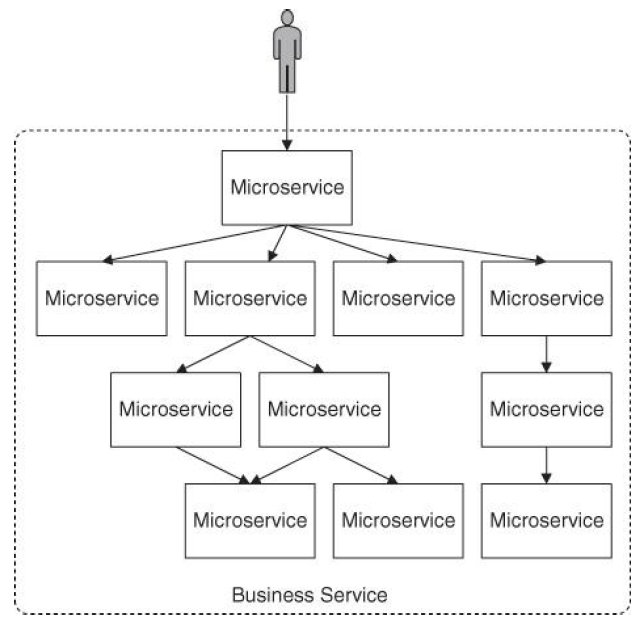
\includegraphics[width=0.5\textwidth]{pictures/businessService.png}
	\caption{Business service}
	\label{aService}
\end{figure}

\subsection{Design Entscheidung}
In diesem Abschnitt wird zunächst das Koordinationsmodell mit den drei Akteuren \textit{Client}, \textit{Service} und \textit{Registry/Load Balancer} vorgestellt. Daraufhin wird auf das Ressourcenmanagement von Instanzen eingegangen. Dazu werden Szenarien vorgestellt, die die Anzahl der Instanzen eines Microservices regulieren. Zum Schluss wird die Arbeitseinteilung und Zuweisung der architektonischen Elemente (Komponenten) erläutert. Dabei werden Möglichkeiten präsentiert, die die Microservice Architektur anbietet und daraufhin welche dieser Möglichkeiten für DevOps geeignet sind.

\subsubsection{Koordinationsmodell}

Beim Koordinationsmodell gibt es drei Akteure. Zum einen die \textit{Registry/Load Balancer}, wobei die Registry für die Verwaltung der Serviceinstanzen zuständig ist und der Load Balancer für die Verteilung der Last auf die verschiedenen Instanzen eines Services. So kann beispielsweise der Load Balancer bei erhöhter Anzahl von Anfragen auf einen Service weitere Instanzen anfordern, sodass Instanzen nicht überlastet werden.\\
Der zweite Akteur ist die \textit{Instanz eines Services}, die Daten beziehungsweise Dienstleistungen anbietet. Die Instanz registriert sich bei der Registry und hinterlegt ihren Namen, Adresse und Interface. Daraufhin steht nun die Instanz für den dritten Akteur bereit: Der \textit{Client} kann dabei ein Benutzer oder ein Service sein, der für einige Aufgaben weitere Services benötigt. Dafür fragt dieser bei der Registry nach den gewünschten Service und erhält die hinterlegten Daten der Serviceinstanz. Mit diesen Daten kann der Client nun die Instanz über das Interface ansprechen und verwenden. Die folgende Abbildung \ref{bService} gibt eine Übersicht der Beziehungen der drei Akteure.

\begin{figure}[htbp]
  \centering
  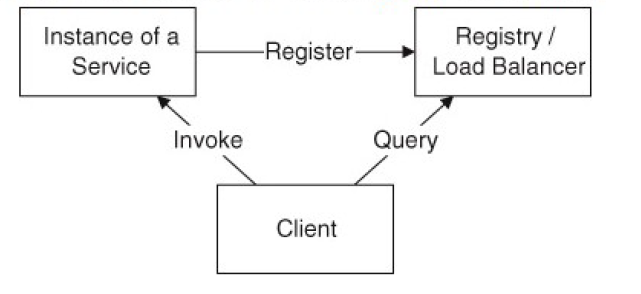
\includegraphics[width=0.5\textwidth]{pictures/3akteure.png}
	\caption{Die drei Akteure der Microservice Architektur}
	\label{bService}
\end{figure}

Da es jederzeit Möglich ist, dass Instanzen ausfallen können oder nicht mehr aktiv sind, ist es wichtig, dass die Registry über diese Instanzen informiert ist. Denn sonst vermittelt die Registry Instanzen an Clienten, die der Client nicht ansprechen kann. Für dieses Problem existiert der Healthcheck. Dabei werden Instanzen nur für eine bestimmte Zeit in der Registry verwaltet. Damit Instanzen nicht aus der Registry entfernt werden, müssen sich die Instanzen periodisch bei der Registry melden. Alternativ kann die Registry proaktive Anfragen an Instanzen stellen, die in der Registry registiert sind. Sollte die Instanz nach bestimmter Zeit keine Antwort liefern wird diese aus der Registry entfernt.

\subsubsection{Ressourcenmanagement}

Ein wichtiger Anforderungspunkt von DevOps ist die Skalierbarkeit. Weitere Serviceinstanzen lassen sich bei Ausfällen von Instanzen oder bei höhere Belastung initialisieren. Auch ist es möglich Instanzen bei geringerer Belastung zu entfernen um so Ressourcen zu sparen. Bei der Entscheidung, welcher Akteur über die Anzahl der Instanzen bestimmt, gibt es drei Szenarien:\\
Zum einen kann der Service selber entschieden ob er von sich weitere Instanzen bereitstellt, dies geschieht wenn der Service erkennt, dass Instanzen überbelastet sind. Zum Anderen kann der Client weitere Instanzen anfordern, sofern dieser bereits im Vorfeld weiss, dass er in naher Zukunft eine erhöhte Anzahl von Anfragen an einen Service hat. Im dritten Szenario kann eine externe Verwaltung durch Monitoring über die Anzahl der Instanzen entscheiden. So kann durch Monitoring erkannt werden, dass zu bestimmten Uhrzeiten ein Service vermehrt verwendet wird. Beispielsweise am Abend oder Wochenende, wo viele Benutzer zuhause sind und der Service von ihnen verwendet wird. 

\subsubsection{Abbildung von architektonischen Elementen}

Bei der Arbeitsaufteilung von Teams, können zum einen mehrere Teams einem Service arbeiten und ein Team an mehreren Services. Dies benötigt allerdings ein erhöhten Koordinationsaufwand. Idealerweise arbeiten an einem Service nur ein Team, wobei ein Team für mehreren Services zuständig sein kann. Dies entspricht auch den Anforderungen von DevOps, das geringe Koordination zwischen den Teams fordert.\\

Neben der Entwicklung einer Komponente von nur einem Team, sollen die Komponenten auch unabhängige Einheiten darstellen. So können diese unabhängig ausgeliefert werden und Änderungen haben keine Auswirkung auf andere Komponenten. Dies verringert ebenfalls die Koordination und beschleunigt die Auslieferung einzelner Komponenten. Die Anforderungen des continuous Deployment des DevOps werden damit ebenfalls erfüllt. 


\subsection{Herausforderungen}

Aufgrund der Eigenschaften, wie geringe Koordination zwischen Teams, hat die Architektur einige Herausforderungen. Dazu zählt zum einen die Systemstabilität und leichte Modifizierbarkeit der Module bei Erkennung von Problemen, wie beispielsweise neuen Versionen von benutzter Dritt-Software. Im folgenden werden die Herausforderungen der Microservicearchitektur genauer betrachtet.

\subsubsection{Systemstabilität}

Clienten sprechen Service über ein Interface an. Diese Interface können sich im Laufe der Entwicklung verändern. Aufgrund der geringen Koordination zwischen den Teams, können Missverständnisse bezüglich der Semantik vom Interface zwischen Client- und Service Team entstehen. So können Services mit neuen Interface einen unerwarteten Input erhalten, oder Clienten von einem Service mit neuen Interface ein unerwarteten Output. Um diesen Problemen entgegenzuwirken ist defensives Programmieren erforderlich, das heißt es benötigt eine große Anzahl unterschiedlicher Exceptions um die Fehler eingrenzen zu können. Zwar ist es möglich bei neuen Änderungen von Services Integrationstests durchzuführen, dies ist allerdings auf Grund der kurzen Releasephasen und der hohen Anzahl von Microservices sehr mühsam und Zeitaufwendig. Daher wird der \textit{Consumer driven contract} verwendet. Für jeden Microservices werden Testcases erstellt, die den Input und Output festlegen. Sobald die Interfacespezifikationen geändert werden, müssen die Testcases angepasst werden und von den Clienten, die den Service verwenden, akzeptiert werden. \\
Ein weitere Punkt für die Sicherstellung der Systemstabilität ist die Korrektheit der Umgebung. Systemumgebungen können fehlerhaft oder falsch konfiguriert sein. Damit der Service dennoch einwandfrei läuft muss bei der Initialisierung die Umgebung geprüft werden und gegebenenfalls muss sich der Service der Umgebung anpassen oder der Service passt die Umgebung an.\\
Ausfälle von Instanzen sind keine Seltenheit. Diese Ausfälle können mit Hilfe von Timeouts ermittelt werden und Clienten müssen alternative Mechanismen bei Timeout bereitstellen und ausführen. 

\subsubsection{Modifizierbarkeit}

Modifizierbarkeit bedeutet, dass Services leicht und schnell auf Änderungen angepasst werden können. Zwar ist es schwer ein Service so robust zu programmieren, dass auf jedes mögliche Problem schnell reagiert werden kann. Dennoch sollte der Service schnell die wahrscheinlichsten Änderungen identifizieren. Dazu gehört die Umgebung eines Services, das auf verschiedenen Rechnern unterschiedlich konfiguriert sein kann. Auch kann sich ein Zustand eines anderen verwendeten Services verändern. Das Interface sowie die angebotene Dienstleistung kann auf einer anderen Art bearbeitet werden, die möglicherweise mehr Zeit in Anspruch nimmt.\\
Neue Versionen von verwendete Bibliotheken und Dritt-Software können ebenfalls veränderte Funktionalität haben und so zu Problemen führen.\\
Da üblicherweise auf Identifizierte Veränderungen nicht direkt reagiert werden kann, wird versucht kaskadierende Effekte so gering wie möglich zu halten, sodass andere Bereiche nicht ebenfalls von den Problemen betroffen werden. Dazu werden mit Hilfe von Modulen die Änderungen gekapselt. Module sind in jeden Service enthalten und lokalisieren sowie isolieren Änderungen. Außerdem bieten die Module ein stabiles Interface zu den Änderungen an, sodass der Service möglichst normal weiterarbeiten kann. 

\subsection{Antipattern}

In diesem Abschnitt werden einige Antipattern vorgestellt und gezeigt wie die korrekte Vorgehensweise ist.

Funktionsumfang eines Services wächst mit der Zeit und den Anforderungen:\\
Services sollten möglichst klein gehalten werden und neu eingeführte Funktionen sollten jeweils ein neuen Service bilden.
Zu wenig Automatisierung der Test und des Deployments:\\
Um kurze Releasephasen einzuhalten ist es wichtig in allen möglichen Bereichen zu automatisieren, da sonst zu viel Zeit verloren geht.\\
Horizontale Schichten werden als Services abgebildet (z.B. Datenschicht und Geschäftslogik):\\
Microservices sollten möglichst unabhängig und einzeln ausführbar sein. Sobald Datenschicht und Geschäftslogik getrennt wird, benötigt mindestens ein Service für den Zugriff auf die Datenbank immer ein anderen Service. Dies entspricht nicht den gewünschten Eigenschaften von Microservices.\\
Jeder Service wird manuell konfiguriert:\\
Muss beispielsweise eine Internetadresse in den Servicen geändert werden, würde es sehr zeitaufwenig sein die Änderungen in jeden Service einzeln auszuführen. Daher sollten die Services mit einem Konfigurationsserver verbunden sein und Änderungen über diesen Server ausgeführt werden.\\
Zu jedem Service existiert nur eine Version:\\
Kurze Releasephasen bedeuten häufige Versionsänderungen. Existiert nur eine Version hat dies zur Folge, dass alle Instanzen der alten Version zerstört werden müssen. Dabei könnten diese Instanzen allerdings gerade von Clienten in Benutzung sein. Daher sollten nur Instanzen durch Serviceinstanzen der neuen Version ersetzt werden, wenn sie nicht verwendet werden.\\




\subsection{Gefahren}

Microservices beinhalten einige Gefahren. Die hohe Anzahl an Netzwerkverbindungen für die Kommunikation zwischen den Servicen, Clienten und der Registy kann zu mögliche Latenzen führen. Wodurch fälschlicherweise Timeouts ermittelt werden können. Auch verschlechtert sich die Effizienz des Business Services, da Clienten länger auf die Antwort eines Services warten muss.\\
Unerwartete Überlastungen von Serviceinstanzen verlangsamen die Performance. Ebenso führen Ausfälle von Instanzen zu geringerer Effizienz der gesamten Anwendung.\\
Bei einer hohen Anzahl von Serviceinstanzen kann es dazu kommen, dass die Registry nicht mit der Verwaltung der Instanzen hinter herkommt und es bei der Vermittlung der Instanzen an die Clienten zu Verzögerungen kommt oder sogar zur falschen Vermittlung einer Instanz.

\subsection{Beispiel}

Ein Beispiel für den Einsatz von Mircoservices ist Netflix. Ihr ganzes Streamingsystem ist auf der Microservicearchitektur aufgebaut. Durch die leichte Skalierbarkeit und Updaten von Microservices im laufenden Betrieb erreicht Netflix eine Verügbarkeitsquote von 99.7\%. Im Schnitt ist Netflix nur zwei Stunden im Monat nicht verfügbar.  


\chapter{Zukunft von DevOps}

\section{Vorraussichtliche Marktakzeptanz}

\section{Organisatorische Probleme}

\section{Prozess Probleme}

\section{Technologische Probleme}

\section{Bugfixing}

\chapter{Zusammenfassung und Fazit}

\end{document}